\documentclass[aspectratio=169,10pt]{beamer}
\usepackage[utf8]{inputenc}
\usepackage[brazil]{babel}
\usepackage{graphicx}
\usepackage{booktabs}

\title{Modelo único vs.\ Ensemble\\na detecção de pneumonia}
\subtitle{2ª Avaliação -- Eletiva de Inteligência Artificial}
\author{Enzo de Barros Nunes \and Guilherme Cardozo de Castro Melo \and Lui Vaz Manso de Queiroz \and Marcelo Bresani Victor de Oliveira \and Matheus de Lucena Henriques \and Thiago de Lima von Sohsten}
\institute{CESAR School --- Recife, PE}
\date{\today}

\begin{document}

\begin{frame}
  \titlepage
\end{frame}

\begin{frame}{Problema e objetivo}
  \begin{itemize}
    \item Classificar radiografias de tórax: normal vs.\ pneumonia.
    \item Três técnicas: \textbf{classificação}, \textbf{transfer learning}, \textbf{ensemble} (alternativa: modelo único).
    \item 30 simulações; inferir H0 ou H1 com teste estatístico ($\alpha=0{,}05$).
  \end{itemize}
\end{frame}

\begin{frame}{Dataset}
  \begin{columns}
    \column{0.45\textwidth}
      \textbf{PneumoniaMNIST} (MedMNIST): 28$\times$28 nativo, redimensionado para 64$\times$64; divisão fixa treino/val/teste.
      \begin{itemize}
        \item Pré-processamento: 3 canais + normalização ImageNet.
        \item Métrica principal: \textbf{F1} (classes desbalanceadas).
      \end{itemize}
    \column{0.55\textwidth}
      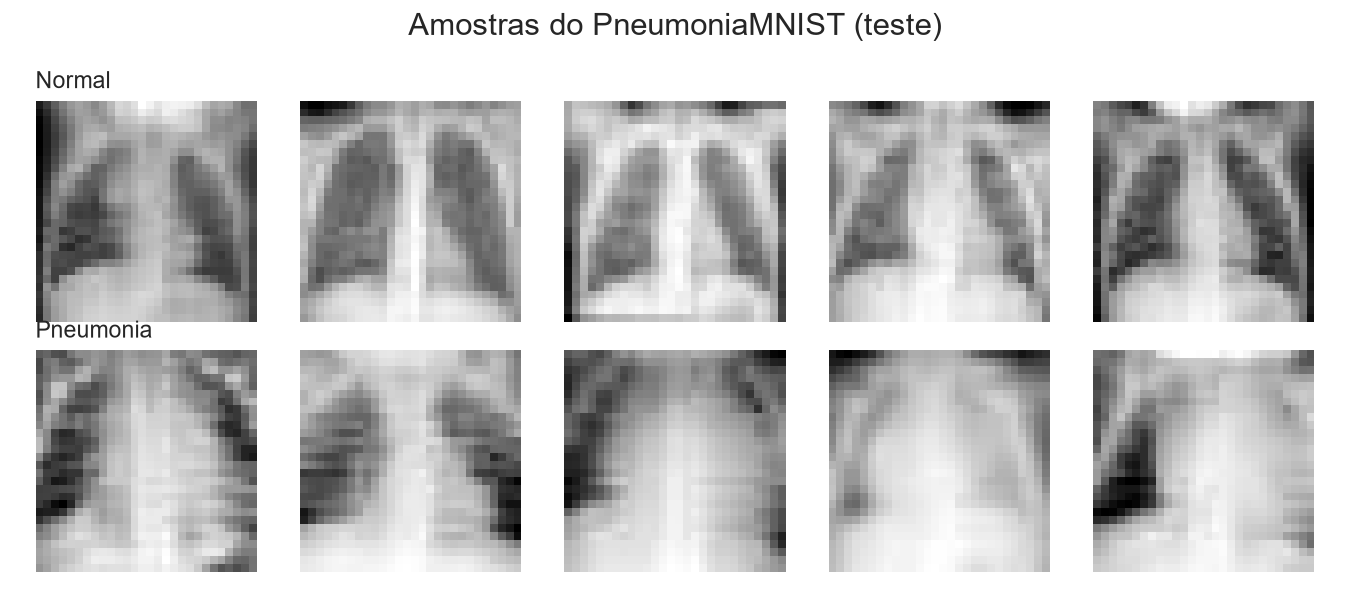
\includegraphics[width=\linewidth]{../results/figs/amostras_dataset.png}
  \end{columns}
\end{frame}

\begin{frame}{Distribuição de classes}
  \centering
  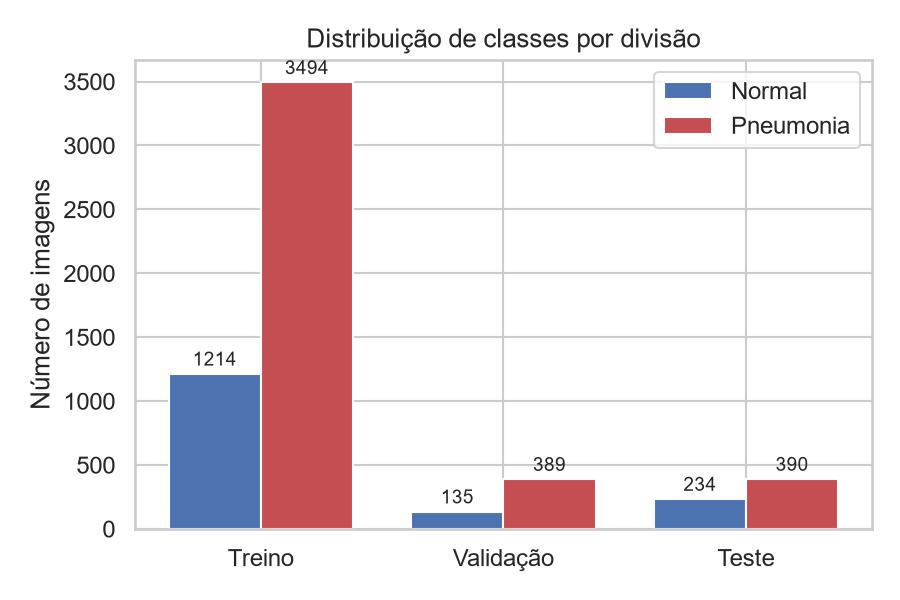
\includegraphics[width=0.62\linewidth]{../results/figs/dist_classes.png}
\end{frame}

\begin{frame}{Cenários comparados}
  \begin{table}
    \centering
    \begin{tabular}{ll}
      \toprule
      & Técnica C \\
      \midrule
      \textbf{H0} (hipótese nula) & ResNet18 único \\
      \textbf{H1} (hipótese alternativa) & Ensemble: ResNet18 + MobileNetV2 + EfficientNet-B0 \\
      \bottomrule
    \end{tabular}
  \end{table}
  Votação suave (média de probabilidades). Mesma ResNet18 treinada em ambos (pareamento).
\end{frame}

\begin{frame}{Pipeline experimental}
  \centering
  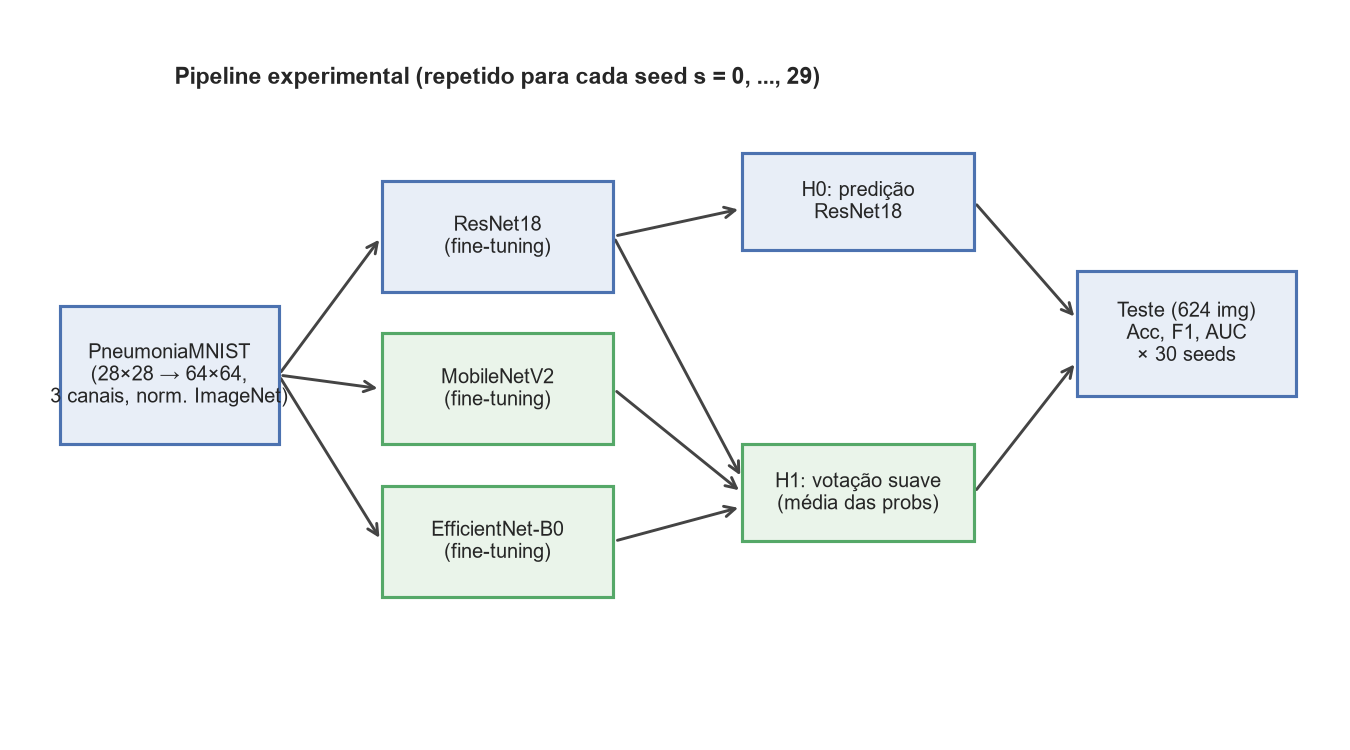
\includegraphics[width=0.82\linewidth]{../results/figs/pipeline.png}
\end{frame}

\begin{frame}{Protocolo experimental}
  \begin{itemize}
    \item Seeds 0--29; Adam, lr $10^{-3}$, batch 128, até 5 épocas + early stopping.
    \item Shapiro-Wilk $\rightarrow$ $t$ pareado ou Wilcoxon (unilateral: H1 $>$ H0).
    \item Cohen's $d$ e gráficos em \texttt{results/figs/}.
  \end{itemize}
\end{frame}

\begin{frame}{Resultados numéricos (30 simulações)}
  \begin{table}
    \centering
    \begin{tabular}{lccc}
      \toprule
      Cenário & Acurácia & F1 & AUC \\
      \midrule
      H0 (modelo único) & 0,8580 $\pm$ 0,0286 & 0,8980 $\pm$ 0,0184 & 0,9691 $\pm$ 0,0093 \\
      H1 (ensemble)     & 0,8690 $\pm$ 0,0118 & \textbf{0,9050 $\pm$ 0,0077} & 0,9677 $\pm$ 0,0074 \\
      \bottomrule
    \end{tabular}
  \end{table}
  \begin{itemize}
    \item H1 vence em \textbf{22 de 30} seeds; dp do F1 cai a menos da metade (0,0184 $\to$ 0,0077).
    \item Tempo de treino: $\approx$21\,s (H0) vs.\ $\approx$85\,s (H1) por simulação ($\approx 4\times$).
  \end{itemize}
\end{frame}

\begin{frame}{F1 por cenário}
  \centering
  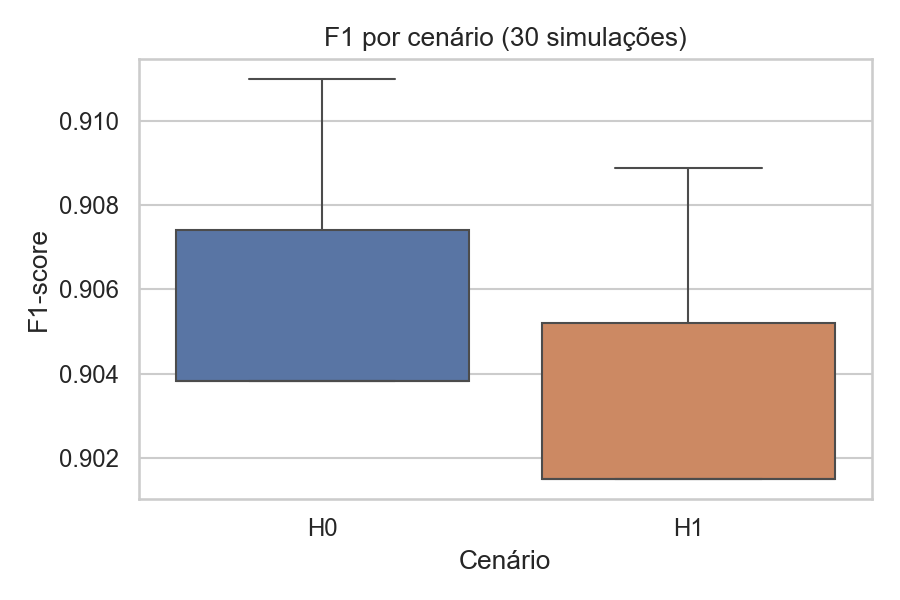
\includegraphics[width=0.75\linewidth]{../results/figs/f1_boxplot.png}
\end{frame}

\begin{frame}{F1 por simulação}
  \centering
  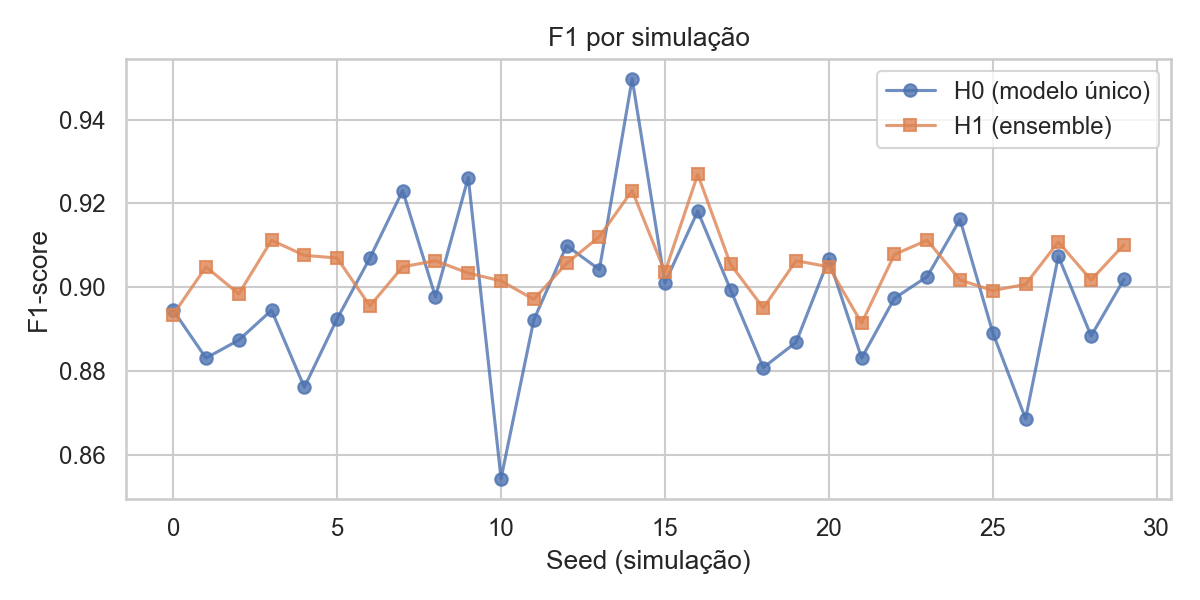
\includegraphics[width=0.85\linewidth]{../results/figs/f1_por_seed.png}
\end{frame}

\begin{frame}{Análise pareada}
  \begin{columns}
    \column{0.5\textwidth}
      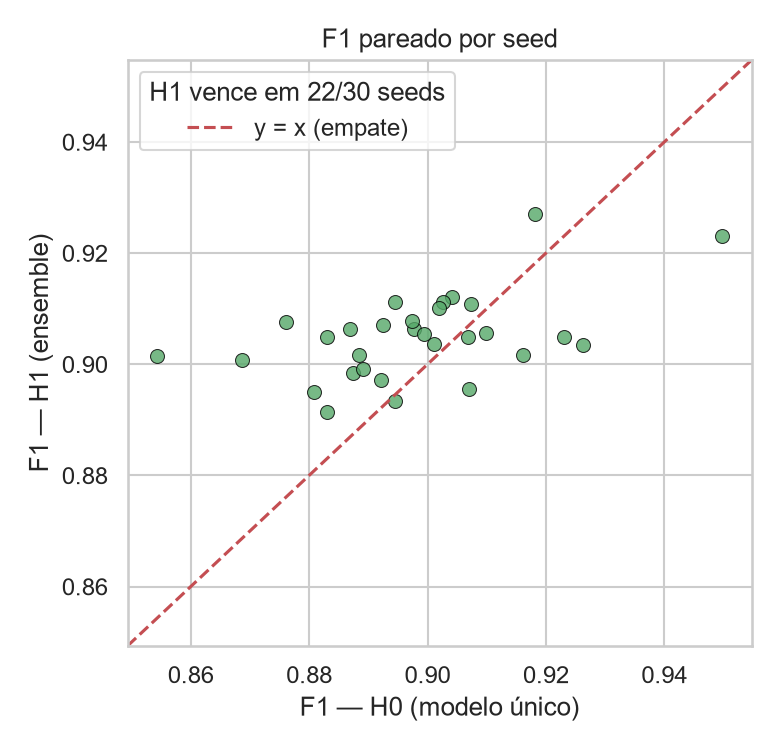
\includegraphics[width=\linewidth]{../results/figs/f1_scatter_pareado.png}
    \column{0.5\textwidth}
      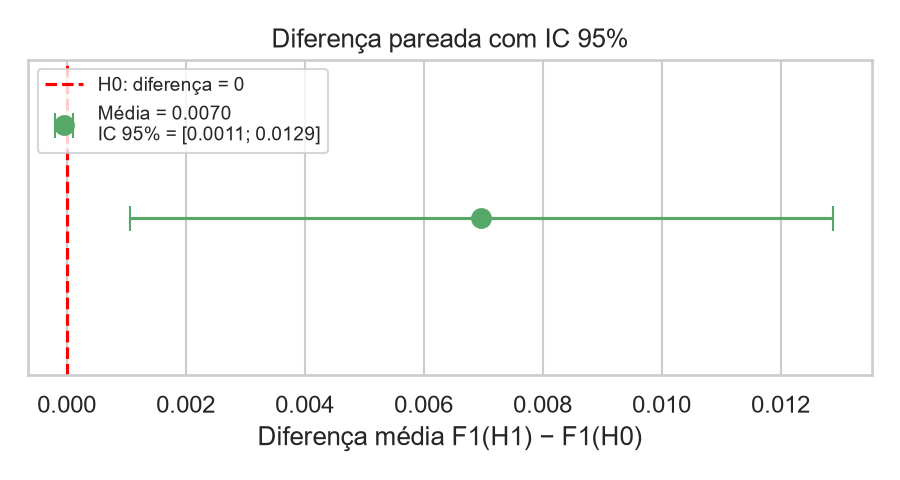
\includegraphics[width=\linewidth]{../results/figs/diff_ic95.png}
  \end{columns}
  \centering
  Diferença média 0,0070; IC 95\% $[0{,}0011;\,0{,}0129]$ exclui o zero.
\end{frame}

\begin{frame}{Diferenças e custo computacional}
  \begin{columns}
    \column{0.5\textwidth}
      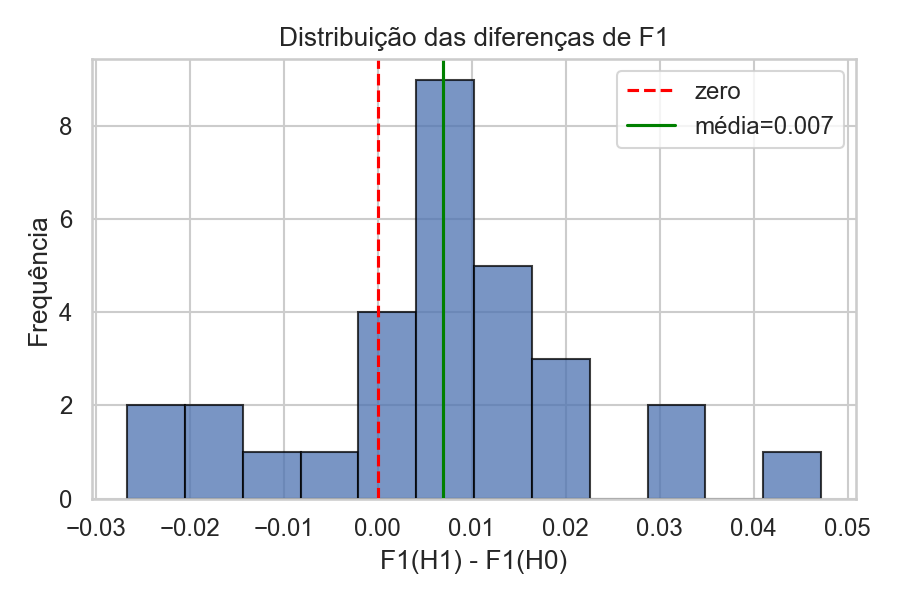
\includegraphics[width=\linewidth]{../results/figs/f1_diff_hist.png}
    \column{0.5\textwidth}
      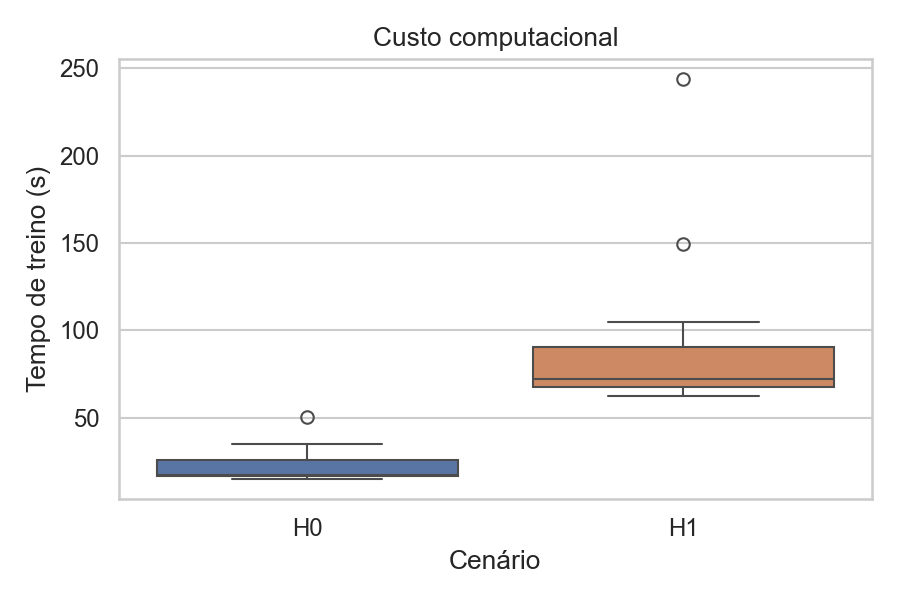
\includegraphics[width=\linewidth]{../results/figs/tempo_treino.png}
  \end{columns}
\end{frame}

\begin{frame}{ROC e matriz de confusão (seed 0)}
  \begin{columns}
    \column{0.5\textwidth}
      \centering
      \textbf{H0}\\
      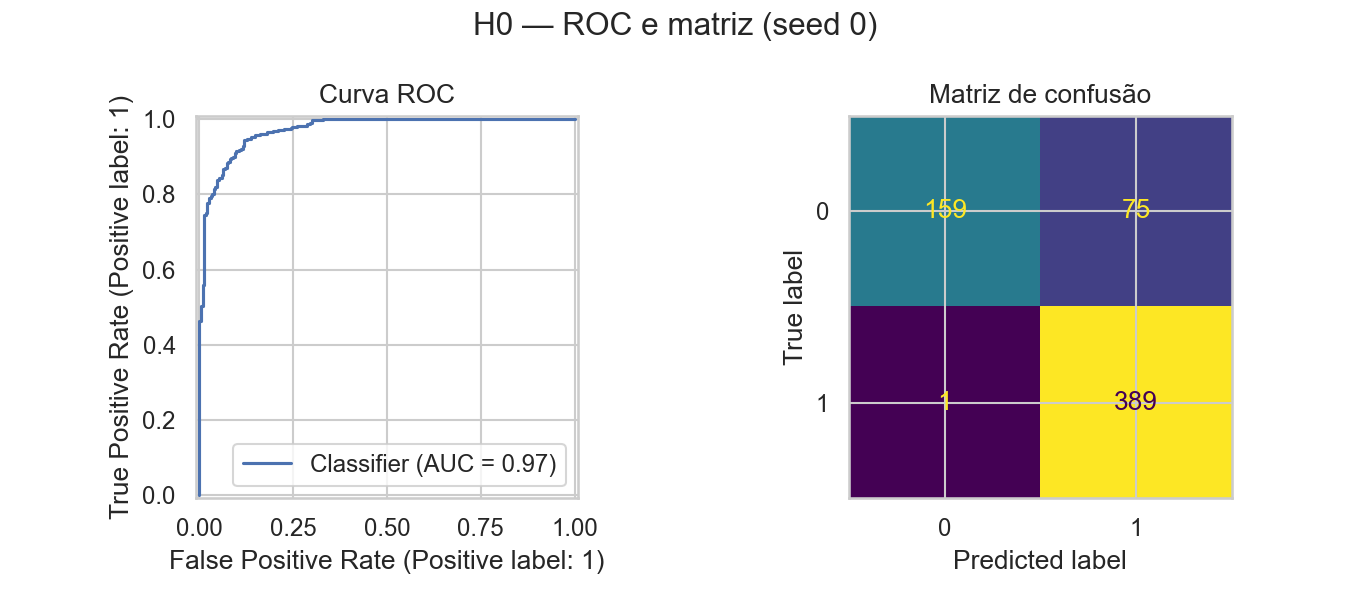
\includegraphics[width=\linewidth]{../results/figs/roc_conf_h0.png}
    \column{0.5\textwidth}
      \centering
      \textbf{H1}\\
      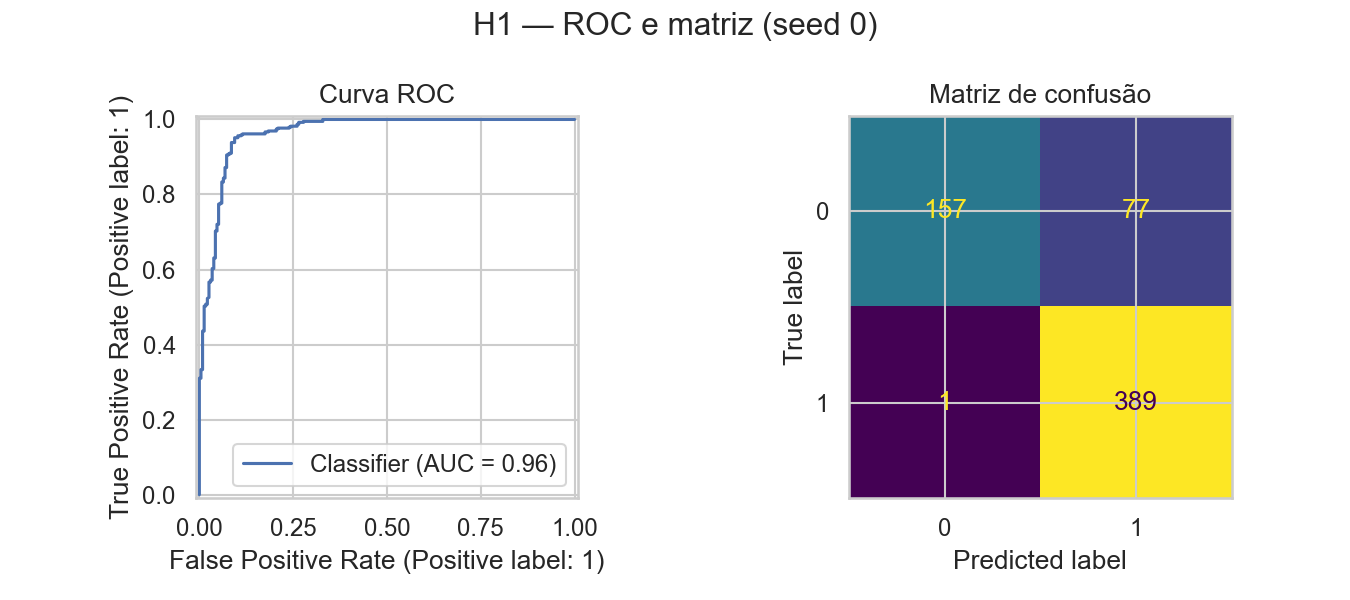
\includegraphics[width=\linewidth]{../results/figs/roc_conf_h1.png}
  \end{columns}
\end{frame}

\begin{frame}{Calibração e limiar de decisão (seed 0)}
  \begin{columns}
    \column{0.5\textwidth}
      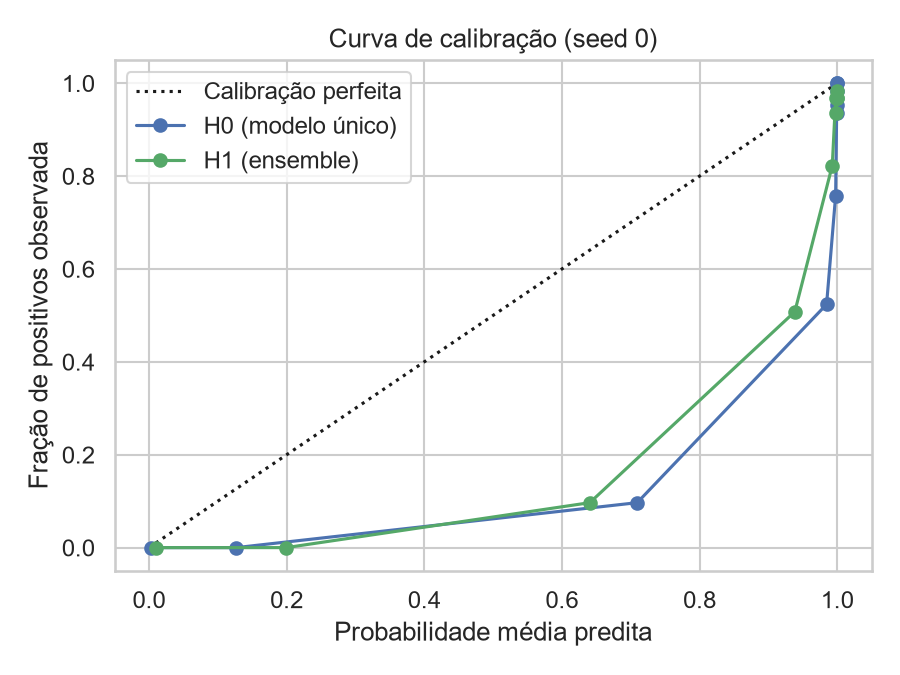
\includegraphics[width=\linewidth]{../results/figs/calibracao.png}
    \column{0.5\textwidth}
      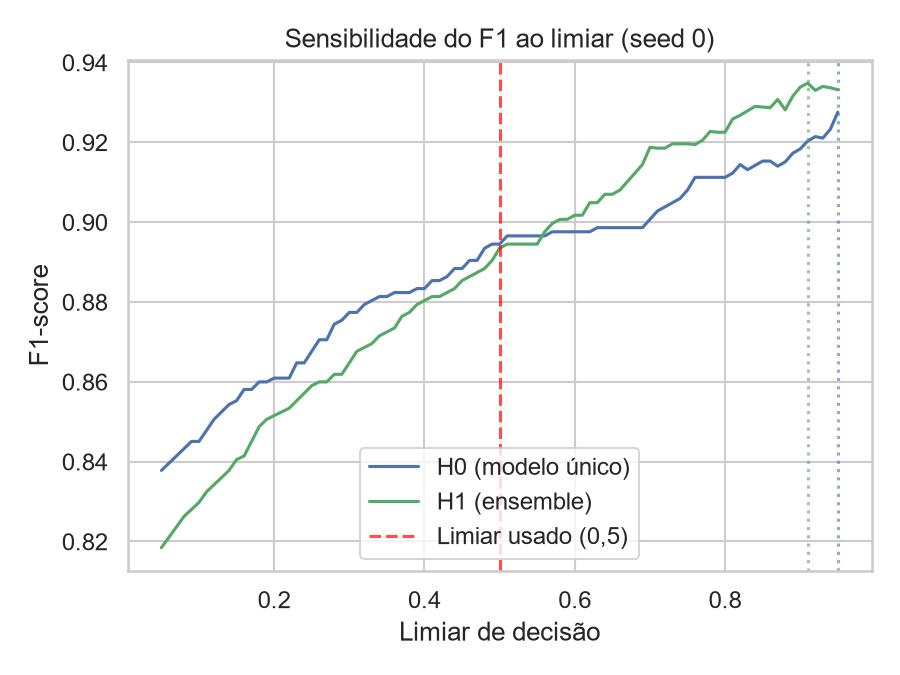
\includegraphics[width=\linewidth]{../results/figs/limiar_f1.png}
  \end{columns}
  \centering
  Zero falsos negativos com limiar 0,5; limiar ótimo $\approx$0,9 elevaria o F1 a $\approx$0,93.
\end{frame}

\begin{frame}{Conclusão estatística}
  \begin{itemize}
    \item Rejeita-se H0: o ensemble (H1) é estatisticamente mais eficaz em F1 (alpha=0,05).
    \item Trade-off: ensemble treina três arquiteturas; tempo de treino tipicamente maior que H0.
  \end{itemize}
\end{frame}

\begin{frame}{Síntese do teste de hipótese}
  \begin{itemize}
    \item Shapiro--Wilk: $W=0{,}9579$, $p=0{,}2739$ $\Rightarrow$ diferenças normais $\Rightarrow$ $t$ pareado.
    \item $t=2{,}41$, $p=0{,}011 < \alpha=0{,}05$ (unilateral) $\Rightarrow$ \textbf{rejeita-se H0}.
    \item Tamanho de efeito: Cohen's $d=0{,}44$ (pequeno a moderado).
    \item Recomendação: H1 quando robustez compensa o custo $4\times$; H0 como baseline rápida.
  \end{itemize}
\end{frame}

\begin{frame}{Demonstração}
  \texttt{python src/simulate.py}\\
  \texttt{python src/finish\_pipeline.py}\\
  \texttt{python src/extra\_plots.py}
\end{frame}

\begin{frame}
  \centering
  \Large Obrigado!\\
  \normalsize Perguntas?
\end{frame}

\end{document}
